\documentclass[]{article}
\usepackage[numbers]{natbib}
\usepackage{amsfonts, amssymb, amsmath}
\usepackage{url}
\usepackage{float}
\usepackage{graphicx}
\usepackage{adjustbox}
\usepackage[colorlinks=true, allcolors=blue]{hyperref}
\usepackage[]{geometry}
\usepackage{url}
\usepackage{tikz, pgfplots}
\usepackage{multicol}
\usetikzlibrary{positioning, shapes.geometric, arrows}

\title{Proposed Funding Models}
\author{
  Thomas, Harper\\
  \texttt{zeroknowledgeltd@gmail.com}
}

\date{\today}

\begin{document}

\maketitle

\section{Funding Rate}

Funding has two dual purposes in the quanto perps market. It is used to incentivise LPs to provide liquidity to the market, and also to protect LPs against directional risk. For the former there is utilisation funding rate, and for the latter a skew funding rate. Each of these are combined to form the total funding that traders are exposed to.

\subsection{Utilisation Funding Rate}

Utilisation funding works as a dynamic cost applied to all traders positions based on current market utilisation and the size of their position. It is paid entirely to LPs. The concept of "funding velocity" is used a price discovery mechanism, by creating a drifting funding rate that moves dependent on market utilisation. As market utilisation moves above 50\%, the funding velocity increases, causing the funding rate to slowly drift upwards until it finds a rate traders are no longer willing to pay.\\

At this point, traders will begin to close their positions causing utilisation to drop, and the utilisation funding rate velocity to go negative. Then over time funding rates slowly decrease, until such a point is reached where trading is suitably cheap for traders and market utilisation increases again. This acts like a PID controller for market utilisation, incentivising partial market utilization at all points.\\

We purposefully do not want a market utilisation of 100\%. This would be bad for traders and LPs. It would mean traders are unable to open new positions, and LPs are unable to exit their positions. It is more preferable the market is always partially utilised, so that there is an ongoing source of yield for LPs, open interest available to traders, and space in the market for LPs to exit. The exact level of optimal market utilisation is a parameter that can be adjusted by governance.\\

% To control the sensitivity and bounds of this mechanism, there are a number of configurable parameters:

\subsection{Model 1}

The simplest model where target utilisation is set at 50\%, and the utilisation funding rate is a linear function of market utilisation.

Configurable parameters:
\begin{enumerate}
\item $maxUtilisationFundingVelocity = I^u_{max}$
\item $minUtilisationFundingRate = i^u_{min}$
\end{enumerate}

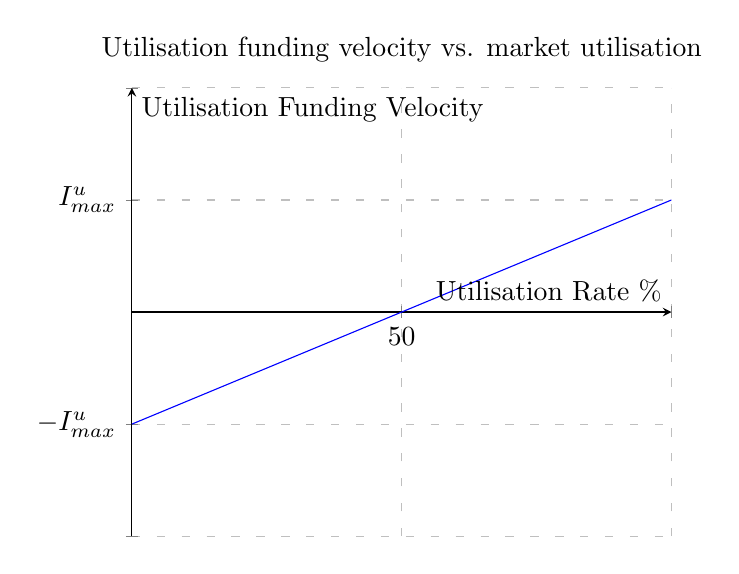
\begin{tikzpicture}
\begin{axis}[
title={Utilisation funding velocity vs. market utilisation},
xmin=-0, xmax=100,
ymin=-50, ymax=50,
axis lines=middle,
xlabel=Utilisation Rate \%,
ylabel=Utilisation Funding Velocity,
xtick={0, 50, 100},
xticklabels={, 50,},
ytick={-50, -25, 0, 25, 50},
yticklabels={, $-I^u_{max}$, , $I^u_{max}$, ,},
ymajorgrids=true,
xmajorgrids=true,
grid style=loosely dashed,
]
\addplot[color=blue, samples=100, domain=0:100]{0.5*x-25};
\end{axis}
\end{tikzpicture}

This system is the most easy to configure, you just set the max velocity and min funding rate. The utilisation funding rate searches for a price that will keep the market utilisation at 50\%. The great thing about this model is it is so simple, and even if we feel the target market utilisation of 50\% is a bit too high or low, we can all adjust OI caps accordingly via the collateralisation ratio.

\subsubsection{Model 1 Math}

$$
\frac{di_u}{dt} = 2 I^u_{max}(uR - 0.5)
$$

$$
utilisationFundingVelocity = 2 \cdot maxFundingVelocity(utilisationRate - 0.5)
$$

$$
i_u = min\left(i^u_{min},\, \frac{i^u_{last} + \frac{di_u}{dt} \cdot (t - t_{last})}{2}\right)
$$
$$
utilisationFundingRate = min(minFundingRate, averageFundingRate)
$$

\subsubsection{Model 2}

This model builds on the last one, adding in a target market utilisation parameter. This allows the system to target a specific market utilisation, say 60\% instead of 50\%. The utilisation funding velocity will then act as a price discovery mechanism to achieve this.

Configurable parameters:
\begin{enumerate}
\item $maxUtilisationFundingVelocity = I^u_{max}$
\item $targetMarketUtilisation = uR_t$
\item $minUtilisationFundingRate = i^u_{min}$
\end{enumerate}

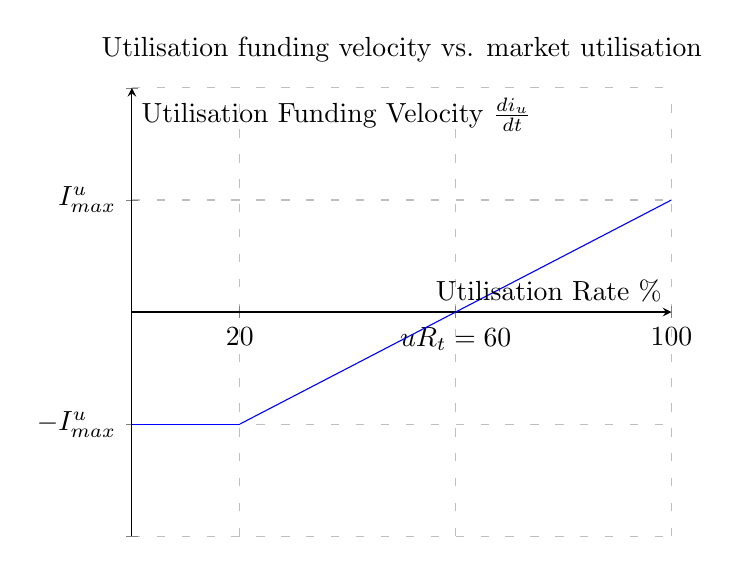
\begin{tikzpicture}
\begin{axis}[
title={Utilisation funding velocity vs. market utilisation},
xmin=-0, xmax=100,
ymin=-50, ymax=50,
axis lines=middle,
% xlabel=$\frac{OI}{V_{max}}$,
xlabel=Utilisation Rate \%,
% ylabel=$\frac{di_u}{dt}$,
ylabel=Utilisation Funding Velocity $\frac{di_u}{dt}$,
xtick={0, 20, 60, 100},
xticklabels={, 20, $uR_t = 60$, 100},
ytick={-50, -25, 0, 25, 50},
yticklabels={, $-I^u_{max}$, , $I^u_{max}$, ,},
ymajorgrids=true,
xmajorgrids=true,
grid style=loosely dashed,
]
\addplot[color=blue, samples=100, domain=20:100]{0.625*x-37.5};
\addplot[color=blue, samples=100, domain=0:20]{-25};
\end{axis}
\end{tikzpicture}

This model is a little more complex than the last one, but it allows us to set a target market utilisation. It is still relatively simple. The crux of whether this added complexity is worth it, is whether we think the target market utilisation is a parameter we want to adjust. The model purposefully assumes that no matter how it is configured, the maximum funding velocity will be achieved at 100\% utilisation, which I believe makes sense.\\

The reason I think we may not need this parameter, is if we wanted to have the same effect as increasing target market utilisation, we would just decrease the collateralisation ratio, increasing OI caps, hence increasing the amount of OI at which point the utilisation funding velocity goes positive.\\

Conversely, what adjusting the target utilisation rate specifically would allow us to do, is adjust the level of OI at which fees to traders start increasing, allowing us an extra lever to increase LP returns.

\subsubsection{Model 2 Math}

$$
\frac{di_u}{dt} = max\left(-I^u_{max}, \frac{I^u_{max}}{1 - uR_t}(uR - uR_t)\right)
$$
$$
utilisationFundingVelocity = max(-maxFundingVelocity, graphLineFundingRate)
$$

$$
i_u = min\left(i^u_{min},\, \frac{i^u_{last} + \frac{di_u}{dt} \cdot (t - t_{last})}{2}\right)
$$
$$
utilisationFundingRate = min(minFundingRate, averageFundingRate)
$$
\subsubsection{Model 3}

This one is the most complex, but also the most flexible. It allows us to specify at what level of utilisation we reach the maximum and minimum utilisation funding rates, but this introduces two new configurable parameters to manage.

Configurable parameters:
\begin{enumerate}
\item $maxUtilisationFundingVelocity = I^u_{max}$
\item $minUtilisationFundingScale = uScale_{max}$
\item $maxUtilisationFundingScale = uScale_{min}$
\item $minUtilisationFundingRate = i^u_{min}$
\end{enumerate}

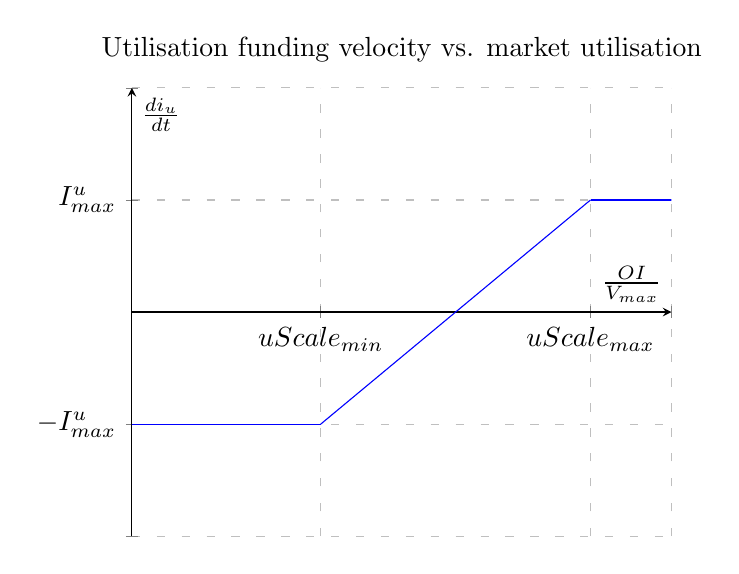
\begin{tikzpicture}
\begin{axis}[
title={Utilisation funding velocity vs. market utilisation},
xmin=-0, xmax=100,
ymin=-50, ymax=50,
axis lines=middle,
xlabel=$\frac{OI}{V_{max}}$,
ylabel=$\frac{di_u}{dt}$,
xtick={0, 35, 85, 100},
xticklabels={, $uScale_{min}$, $uScale_{max}$,},
ytick={-50, -25, 0, 25, 50},
yticklabels={, $-I^u_{max}$, , $I^u_{max}$, ,},
ymajorgrids=true,
xmajorgrids=true,
grid style=loosely dashed,
]
\addplot[color=blue, samples=100, domain=35:85]{x-60};
\addplot[color=blue, samples=100, domain=85:100]{25};
\addplot[color=blue, samples=100, domain=0:35]{-25};
\end{axis}
\end{tikzpicture}

I am not an advocate for this model. I am not sure why we would need the ability to the utilisation rate at which both the minimum and maximum funding velocities are achieved. It does give us more control over funding velocity than previous models, but it introduces an extra configurable variable and is less intuitive to understand. The reason I came up with this in the first place is it mirrors how skew scale works for skew funding in synthetix v3.

\end{document}
